\id{МРНТИ 49.33.29; 28.23.37}{https://doi.org/10.58805/kazutb.v.2.27-710}

\begin{articleheader}
\sectionwithauthors{Б.Н. Жоламанов, М.К. Нұрғалиев, А.Б. Болатбек, Қ.Т. Көпбай, Д.А. Қожабек}{SINGLE ANCHOR NODE POSITIONING METHOD USING ANTENNA ARRAY AND MACHINE LEARNING}

{\bfseries
B.N. Zholamanov\alink{https://orcid.org/0000-0001-8206-7425}\textsuperscript{\envelope },
M.K. Nurgaliyev\alink{https://orcid.org/0000-0002-6795-5384},
A.B. Bolatbek\alink{https://orcid.org/0009-0004-7613-5507},
K.T. Kopbay\alink{https://orcid.org/0000-0003-1583-2099},
D.A. Kozhabek\alink{https://orcid.org/0009-0007-8720-8734}
}
\end{articleheader}

\begin{affiliation}
Al-Farabi Kazakh National University, Almaty, Kazakhstan

\raggedright \textsuperscript{\envelope }Корреспондент-автор: zholamanov.batyrbek@kaznu.kz
\end{affiliation}

Positioning is a fundamental process in wireless sensor networks (WSNs)
and Internet of Things (IoT) systems to accurately track the location of
nodes. This study presents a cost-effective and scalable single-anchor
node positioning system integrating ZigBee technology, directional
antennas, and machine learning (ML). The system utilizes a
custom-designed directional antenna array and machine learning
algorithms to process Received Signal Strength Indicator (RSSI) data,
achieving precise localization with minimal hardware requirements.
Experimental results confirm the superiority of the antenna array,
demonstrating a maximum gain of 10 dBi and enhanced signal reception
compared to monopole and single-patch antennas. The XGBoost model
achieved high accuracy, with R² values of 97.76\% on training and
90.95\% on test data.

{\bfseries Keywords:} Wireless Sensor Networks, ZigBee technology, node
positioning, RSSI, directional antenna, machine learning.

\begin{articleheader}
{\bfseries АНТЕННА МАССИВІ МЕН МАШИНАЛЫҚ ОҚЫТУДЫ ҚОЛДАНУ АРҚЫЛЫ БІР ЯКОРЛЫ
ТҮЙІНГЕ НЕГІЗДЕЛГЕН ПОЗИЦИЯЛАУ ӘДІСІ}

{\bfseries
Б.Н. Жоламанов\textsuperscript{\envelope },
М.К. Нұрғалиев,
А.Б. Болатбек,
Қ.Т. Көпбай,
Д.А. Қожабек
}
\end{articleheader}

\begin{affiliation}
әл-Фараби атындағы Қазақ Ұлттық Университеті, Алматы, Қазақстан,

e-mail: zholamanov.batyrbek@kaznu.kz
\end{affiliation}

Позициялау - сымсыз сенсорлық желілердегі (WSN) және IoT жүйелеріндегі
түйіндердің орналасуын дәл бақылау үшін негізгі процесс болып табылады.
Зерттеу барысында ZigBee технологиясын, бағытталған антенналарды және
машиналық оқытуды (ML) біріктіретін бір якорлық түйінді пайдаланып
үнемді және масштабталатын позициялау әдісін ұсынылды. Жүйе ең аз жабдық
талаптары үшін дәл орналасуды қамтамасыз ете отырып, арнайы әзірленген
антенналық торды және машиналық оқыту алгоритмдерін қабылдайтын сигнал
деңгейінің индикаторы (RSSI) деректерін өңдеу үшін пайдаланады.
Эксперименттік нәтижелер монопольді және бір патч антенналарымен
салыстырғанда, 10 дБи максималды күшейтуді және сигнал қабылдауды
жақсартатын антенналық тордың артықшылықтарын растайды. XGBoost моделі
оқыту деректерінде 97,76\% және тестілеу деректерінде 90,95\%
R\textsuperscript{2} детерминант коэффициенттерімен жоғары дәлдікке қол
жеткізді.

{\bfseries Түйін сөздер:} сымсыз сенсорлық желілер, ZigBee технологиясы,
түйінді позициялау, RSSI, антенналық тор, машиналық оқыту.

\begin{articleheader}
{\bfseries МЕТОД ПОЗИЦИОНИРОВАНИЯ НА ОСНОВЕ ОДНОГО ЯКОРНОГО УЗЛА С
ИСПОЛЬЗОВАНИЕМ АНТЕННОЙ РЕШЕТКИ И МАШИННОГО ОБУЧЕНИЯ}

{\bfseries
Б.Н. Жоламанов\textsuperscript{\envelope },
М.К. Нұрғалиев,
А.Б. Болатбек,
Қ.Т. Көпбай,
Д.А. Қожабек
}
\end{articleheader}

\begin{affiliation}
Казахский национальный университет имени аль-Фараби, Алматы, Казахстан,

e-mail: zholamanov.batyrbek@kaznu.kz
\end{affiliation}

Позиционирование является основным процессом в беспроводных сенсорных
сетях (WSN) и системах Интернета вещей (IoT) для точного отслеживания
местоположения узлов. В данном исследовании представлен экономичный и
масштабируемый метод позиционирования с использованием одного якорного
узла, который объединяет технологию ZigBee, направленные антенны и
машинное обучение (ML). Система использует специально разработанную
антенную решетку и алгоритмы машинного обучения для обработки данных
индикатора уровня принимаемого сигнала (RSSI), обеспечивая точное
позиционирование при минимальных требованиях к оборудованию.
Экспериментальные результаты подтверждают преимущества антенной решетки,
демонстрируя максимальный коэффициент усиления 10 дБи и улучшенный прием
сигнала по сравнению с монопольными и одиночными патч-антеннами. Модель
XGBoost достигла высокой точности с коэффициентами детерминации R²
97,76\% на обучающих данных и 90,95\% на тестовых данных.

{\bfseries Ключевые слова:} беспроводные сенсорные сети, технология ZigBee,
позиционирование узлов, RSSI, антенная решетка, машинное обучение.

\begin{multicols}{2}
{\bfseries Introduction.} Wireless Sensor Networks are an integral part of
modern applications, including environmental monitoring, disaster
management, and the IoT. Accurate node localization is crucial for these
applications as it directly affects the relevance and usability of the
collected data {[}1{]}.

In open environments and small-scale deployments, where issues like
interference and noise are minimized, traditional methods such as GPS
and multi-anchor node systems are widely used {[}2{]}.

GPS-based localization offers high accuracy and global coverage but is
often unsuitable for small-scale deployments due to its cost and energy
consumption requirements {[}3-4{]}. Continuous operation of the GPS
module significantly drains the battery of sensor nodes, which is a
critical limitation in WSNs with constrained resources. Additionally,
integrating GPS increases the size and complexity of sensor nodes,
making it an impractical choice for compact or lightweight designs.

The study {[}5{]} investigates 3D indoor positioning in multi-story
buildings using Ultra-Wideband (UWB) technology, focusing on the impact
of multiple anchors on positioning accuracy and performance improvement.
The study {[}6{]} examines the impact of multiple anchors in 3D indoor
positioning using UWB technology, highlighting the effectiveness of
Particle Swarm Optimization (PSO) in reducing Non-Line-of-Sight (NLOS)
errors from 33 cm to 10 cm and significantly enhancing system accuracy
under NLOS conditions. Multi-anchor node systems, while effective in
many cases, present their own challenges. The need for multiple
stationary reference nodes increases the cost of equipment and
deployment, even for small-scale networks. Moreover, the complexity of
communication and data exchange between anchor nodes reduces scalability
and performance over time. These systems may also require meticulous
maintenance and calibration, which can be challenging in remote or open
environments.

An alternative approach involves single-anchor node systems equipped
with directional antennas and ML methods. Positioning systems that use
single-anchor nodes and directional antennas have been actively studied
to reduce hardware costs and simplify deployment compared to traditional
multi-anchor systems. Directional antennas are advantageous as they
provide angular information critical for position estimation. For
instance, Yong Fu et al. proposed a real-time algorithm for WSN using an
antenna array to estimate the direction of arrival (DoA) combined with
RSSI values {[}7{]}. While achieving sub-meter accuracy in controlled
environments, the method showed significant sensitivity to multipath
interference. Other approaches, like those by Wang et al., employed
mechanically rotating directional antennas for angular position
calculation. However, these systems introduced latency due to mechanical
movements and required precise synchronization, limiting their usability
in real-time applications {[}8{]}. ML methods have also been employed to
improve localization accuracy by identifying complex patterns in signal
data. Groth et al. introduced a calibration-free system that used a
random forest model with RSSI data to map spatial coordinates {[}9{]}.
While the system was effective without extensive environmental
calibration, it faced challenges with dynamic RSSI variations. Hybrid
systems that combine directional antennas with advanced statistical or
ML models aim to address these limitations. For instance, Schmidt et al.
developed the SALOS system, which utilizes UWB signals and statistical
propagation models to achieve high accuracy even under multipath
propagation conditions {[}10{]}. However, its reliance on expensive UWB
equipment has limited its broader adoption.

Numerous studies have been conducted using ZigBee technology for indoor
localization tasks. The paper {[}11{]} examines a localization algorithm
for a mobile robot in complex indoor environments using a ZigBee
wireless network. An improved algorithm based on RSSI and the least
squares method reduced the positioning error from 1.59 m to 0.66 m. The
paper {[}12{]} focuses on the development of an indoor localization
system using ZigBee modules and a 3D trilateration algorithm to
determine the positions and distances between unknown nodes. To enhance
accuracy, a Kalman filter and signal propagation parameter optimization
are applied, reducing the average localization error from 0.6389 m to
0.16 m with optimal reader placement at a height of 2.5 m. The paper
{[}13{]} introduces the MuCHLoc system, which leverages radio frequency
fingerprints and multi-channel RSS measurements to improve localization
accuracy. The method compensates for RSS instability by utilizing
differences in signals across ZigBee channels, improving accuracy by
15\% and effectively operating in dynamic environments.

This study introduces a novel single-anchor node localization system
that leverages ZigBee technology, directional antennas, and machine
learning to address the limitations of traditional multi-anchor setups.
By integrating a directional antenna array with machine learning
algorithms, the system demonstrates significant improvements in signal
reception and localization accuracy. The proposed approach minimizes
hardware costs, simplifies deployment, and provides a scalable,
energy-efficient alternative for WSN, particularly in
resource-constrained environments.

The novelty of the system lies not in the individual use of ZigBee,
directional antennas, or machine learning - each of which has been
previously investigated - but in the specific combination and
implementation of these components in a single-anchor setup. To the best
of our knowledge, this is the first study to use a custom-designed
four-element patch antenna array with ZigBee modules combined with
machine learning to improve localization performance using only a single
anchor node. Previous approaches have relied either on multiple anchors,
mechanically rotating antennas, or expensive technologies. In contrast,
our system offers a practical, low-cost solution that maintains high
localization accuracy without the drawbacks of mechanical movement,
calibration complexity, or high hardware cost, making it particularly
suitable for scalable deployment in industrial, agricultural, or remote
settings.

{\bfseries Materials and methods.}

\emph{{\bfseries 2.1 Experimental setup}}

The experiment was conducted in an open field without any obstacles to
minimize the impact of radio wave interference, which occurs due to the
superposition of multiple waves. Figure 1 shows the experimental area,
demonstrating a flat, unobstructed area free from unwanted factors.

\begin{figure}[H]
	\centering
	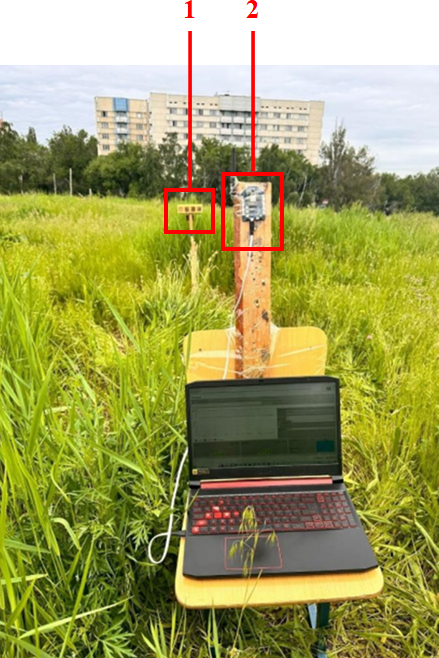
\includegraphics[width=0.35\textwidth]{media/ict/image41}
	\caption*{Fig.1- Experimental area.1 - Transmitter module with patch
antenna; 2 - Receiver module}
\end{figure}

To measure RSSI values, the XCTU software was used in conjunction with
XBee modules (Figure 1). One module, equipped with a monopole antenna,
was connected to a laptop and served as the receiver. The other module,
fitted with a directional antenna array, acted as the transmitter. After
connecting the two devices via the XCTU interface, signal transmission
was configured, and RSSI values received by the antenna array were
recorded. The primary goal of the experiment was to measure RSSI at
various distances and angular positions relative to the antenna, with
the collected data intended for machine learning tasks.

Measurements were taken at distances of 2 m, 5 m, 10 m, 15 m, and 20 m.
The angle range varied from −10° to 190° in 10° increments, resulting in
a total of 200 angular positions. To ensure the accuracy of the
experiment, each angle and distance was fixed with maximum antenna
stability.

\emph{{\bfseries 2.2. Experimental devices.}} For the experiment, Digi XBee
wireless modules were utilized to ensure reliable connectivity and data
transmission. XBee modules support various wireless communication
standards, including Zigbee, 802.15.4, Wi-Fi, and cellular technologies
such as 3G/4G/LTE, making them a versatile solution for a wide range of
applications.

These modules are widely used in IoT systems, industrial automation,
smart agriculture, home automation, and telemetry. The XBee radio module
used in this experiment is depicted in Figure 1, and its key technical
specifications are outlined below in table 1.
\end{multicols}

\tcap{Table 1 - Technical specifications}
\begin{longtblr}[
  label = none,
  entry = none,
]{
  cells = {c},
  hlines,
  vlines,
}
\textbf{Parameter} & \textbf{Specification}\\
Data
			Rate & 250
			Kbps for radio signals; up to 1 Mbps for analog signals\\
Range & Up
			to 60 m in indoor/urban environments; up to 1200 m in open areas\\
Transmission
			Power & +8
			dB\\
Receiver
			Sensitivity & −103
			dB (1\% error rate)\\
Supply
			Voltage & 2.1–3.6
			V\\
Current
			Consumption & 135
			mA during transmission (19 dBm); 17 mA during reception
\end{longtblr}

\begin{multicols}{2}
A directional antenna array, consisting of four patch antennas, was
chosen for this experiment. The use of such an array was essential
because the experiment could not be performed effectively with a
monopole antenna, like the one used in the transceiver. Monopole
antennas provide omnidirectional radiation, which results in RSSI values
that depend solely on the distance between the transmitter and receiver.
This characteristic makes it impossible to determine the directional
orientation of the transmitter relative to the directional antenna.

To address this limitation, microstrip patch antennas with an air gap
were designed, simulated, and subsequently fabricated for use in the
array. These antennas were selected for their compact size and
compatibility with modern wireless communication systems, including
Wi-Fi, mobile networks, and satellite communication.

\emph{{\bfseries 2.3. Designing a patch antenna using MATLAB antenna
toolbox.}} The shape of a patch antenna can vary widely, taking forms
such as square, circular, or rectangular, depending on the design goals
and application requirements. For this experiment, the geometric
parameters of the patch antenna were determined using the MATLAB Antenna
Toolbox.

This tool enables precise optimization of antenna dimensions to achieve
the desired performance characteristics. Specifically, the parameters
were chosen to minimize the \emph{S\textsubscript{11 \hspace{0pt}}}
parameter, which represents the reflection coefficient and indicates
efficient power transfer. Alternatively, formulas (1-5), can also be
used to design patch antennas for specific operational frequencies. The
geometric dimensions of the designed patch antenna are presented in
Figure 2. The antenna was constructed from three primary components:

- \emph{Conductive Patch:} The patch serves as the radiating element and
is typically made of copper due to its high conductivity, although
other metals may be used. The geometry of the patch directly affects
the operating frequency, enabling customization for specific
applications.

- \emph{Dielectric Substrate:} The substrate is located beneath the
conductive patch and isolates it from the ground plane. For this
design, an \emph{FR-4} fiberglass epoxy laminate with a dielectric
constant ε = 4,4 was chosen. This material influences signal
propagation speed and impedance.

- \emph{Ground Plane:} The ground plane is positioned on the opposite
side of the substrate. It directs the radiated signal, ensuring it
propagates in a specific direction. A coaxial feed line is used to
provide power to the patch via the ground plane.
To ensure compatibility with the XBee module operating under the ZigBee
protocol, which spans a wide frequency range with 16 channels spaced 5
MHz apart, the antenna includes an air gap to enhance performance. This
design ensures optimal impedance matching and effective radiation across
the required frequency bands.

\begin{figure}[H]
	\centering
	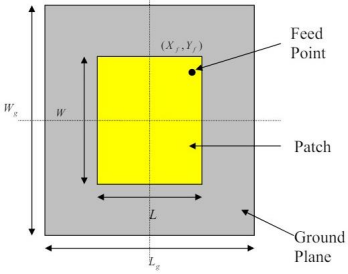
\includegraphics[width=0.4\textwidth]{media/ict/image42}
	\caption*{Fig.2 - Geometrical parameters of the patch antenna}
\end{figure}

The width of the microstrip patch antenna is calculated using Equation
(1):

\begin{equation}
W = \frac{c}{2f_{0}\sqrt{\frac{\varepsilon_{r} + 1}{2}}}
\end{equation}

where:

- \(W\): Width of the patch;

- \(c\): Speed of light;

- \(f_{0}\)\hspace{0pt}: Operating frequency;

- \(\varepsilon_{r}\)\hspace{0pt}: Dielectric constant of the substrate.

To calculate the length, the following intermediate parameters are
required:


1. \emph{Effective dielectric constant} (\(\varepsilon_{reff}\)) is
calculated using Equation (2):

\begin{equation}
\varepsilon_{reff} = \frac{\varepsilon_{r} + 1}{2} + \frac{\varepsilon_{r} - 1}{2}\left\lbrack 1 + \frac{12h}{W} \right\rbrack^{- \frac{1}{2}}
\end{equation}

where: \(h\) - thickness of the dielectric substrate.

2. \emph{Effective length} (\(L_{eff}\)) is determined by Equation (3):

\begin{equation}
L_{eff} = \frac{c}{2f_{0}\sqrt{\epsilon_{reff}}}
\end{equation}

3. \emph{Extension in length} (ΔL) is obtained from Equation (4):

\begin{equation}
\mathrm{\Delta}L = 0.412h\frac{(\varepsilon_{reff} + 0.3)(\frac{W}{h} + 0.264)}{(\varepsilon_{reff} - 0.258)(\frac{W}{h} + 0.8)}
\end{equation}

4. \emph{The actual length} (L) of the patch is computed as:

\begin{equation}
L = L_{eff} - 2\mathrm{\Delta}L
\end{equation}

\emph{{\bfseries 2.4. Machine learning techniques.}} After collecting the
data, it was processed and analyzed using machine learning techniques
like XGBoost, Random Forest, SVM and KNN.

XGBoost is a powerful tool for addressing tasks involving regularized
gradient boosting, an effective ensemble learning method designed to
improve prediction accuracy {[}14{]}. Ensemble methods, such as gradient
boosting, combine the outputs of multiple models to produce stable and
accurate predictions.

Random Forest is an ensemble machine learning method based on using
multiple decision trees for classification or regression. It has high
robustness to outliers and overfitting due to the random selection of
features and data when constructing trees.

Support Vector Machine is a method that uses a hyperplane to separate
classes with the maximum margin between them. SVM is particularly
effective for tasks with small datasets and works well with both
linearly and non-linearly separable data using kernel functions.

k-Nearest Neighbors (k-NN) is a method that classifies objects based on
their proximity to the k nearest neighbors in the feature space. The
algorithm is simple to implement but is sensitive to the sample size and
the choice of distance metric.

The performance of the model was evaluated using four key metrics: Mean
Squared Error, Root Mean Squared Error, Coefficient of Determination and
Mean Absolute Error.

\emph{Mean Squared Error (MSE):} This loss function is used to measure
the average squared difference between actual and predicted values, as
shown in Equation (6):

\begin{equation}
L\left( y,\widehat{y} \right) = \frac{1}{2}\sum_{i = 1}^{n}{{(y_{i} - {\widehat{y}}_{i})}^{2}\ }
\end{equation}

where:

- \(y_{i}\): Actual value.

- \({\widehat{y}}_{i}\): Predicted value.

- \(n\): Number of data points.

\emph{Root Mean Squared Error (RMSE):} This loss function is used to
measure the square root of the average squared difference between actual
and predicted values, as shown in Equation (7)

\begin{equation}
RMSE = \sqrt{\frac{1}{n}\sum_{i = 0}^{n - 1}{(y_{i} - {\widehat{y}}_{i})}^{2}}
\end{equation}

where:

- \(y_{i}\): Actual value.

- \({\widehat{y}}_{i}\)\hspace{0pt}: Predicted value.

- \(n\): Number of data points.

\emph{Coefficient of Determination (R\textsuperscript{2}):} This metric
evaluates how well the model explains the variance in the target
variable. It is expressed as:

\begin{equation}
R^{2} = 1 - \frac{{SS}_{res}}{{SS}_{tot}}
\end{equation}

where:

- \({SS}_{res}\) is the residual sum of squares.

- \({SS}_{tot}\) is the total sum of squares.

\emph{Mean Absolute Error (MAE):} This loss function measures the
average absolute difference between actual and predicted values, as
shown in Equation (9):

\begin{equation}
MAE = \frac{1}{n}\sum_{i = 0}^{n - 1}{(|y_{i} - {\widehat{y}}_{i}|)}
\end{equation}

where:

- \(y_{i}\): Actual value.

- \({\widehat{y}}_{i}\): Predicted value.

- \(n\): Number of data points.

{\bfseries Results and Discussion.} To improve the gain of a single patch
antenna, an antenna array consisting of four patch antennas was
assembled, as shown in Figure 3.

\begin{figure}[H]
	\centering
	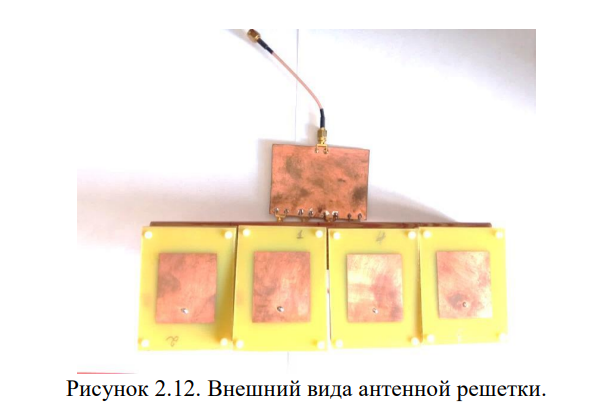
\includegraphics[width=0.4\textwidth]{media/ict/image43}
	\caption*{Fig.3 - The appearance of the patch antenna}
\end{figure}

During initial experiments, it was determined that the gain of a single
patch antenna was insufficient, leading to packet loss during
transmission and reception between isotropic and directional antennas.
By configuring all antennas in the array to operate in phase, the
signals emitted by each antenna constructively interfere in the desired
direction, resulting in increased gain. Simultaneously, signals in other
directions destructively interfere, reducing unwanted radiation.
Achieving proper phase alignment within the array was critical to
maximize the gain in the desired direction while minimizing signal
strength in other directions. This was accomplished through precise
placement and phase delay adjustments for each antenna in the array.

The reflection coefficient (S\textsubscript{22}) of the antenna array
was studied in the frequency range from 2.2 to 2.7 GHz. The Figure 4
shows that the minimum value of the reflection coefficient, equal to
approximately -40 dB, is achieved at a frequency of 2.56 GHz, which
indicates the best matching of the antenna at this point. At the same
time, the reflection coefficient values \hspace{0pt}\hspace{0pt}remain
quite low throughout the analyzed frequency range, which makes the
antenna suitable.
\end{multicols}

\begin{figure}[H]
   \centering
   \begin{subfigure}{0.49\textwidth}
   	\centering
   	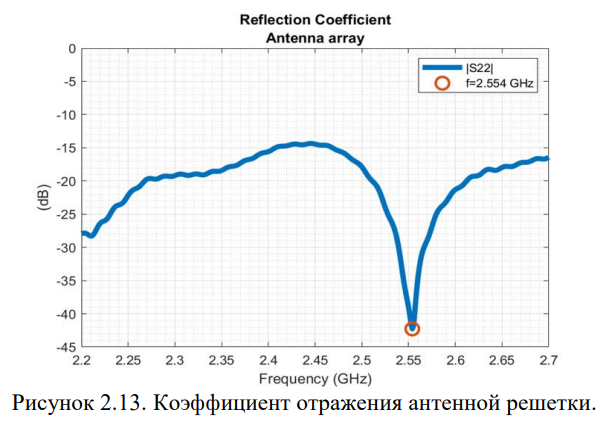
\includegraphics[width=\textwidth]{media/ict/image44}
   	\caption*{Fig.4 - The reflection coefficient of the antenna array}
   \end{subfigure}
   \begin{subfigure}{0.45\textwidth}
   	\centering
   	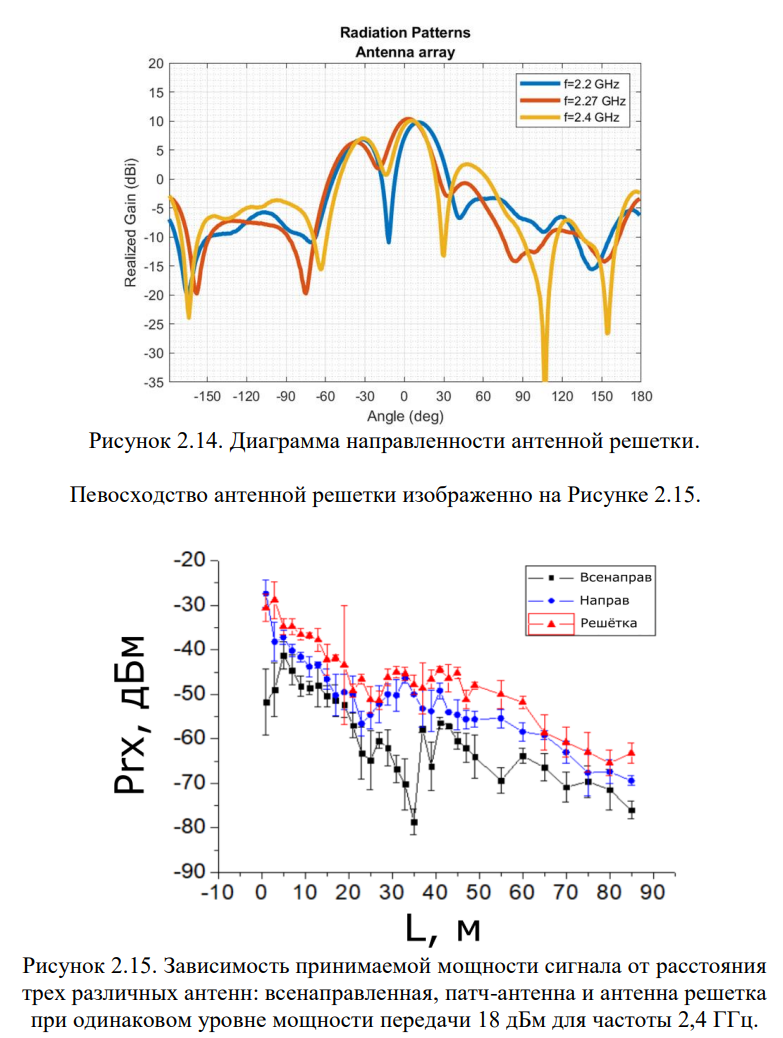
\includegraphics[width=\textwidth]{media/ict/image45}
   	\caption*{Fig.5 - The radiation patterns of the antenna}
   \end{subfigure}
   \begin{subfigure}{0.5\textwidth}
       \centering
       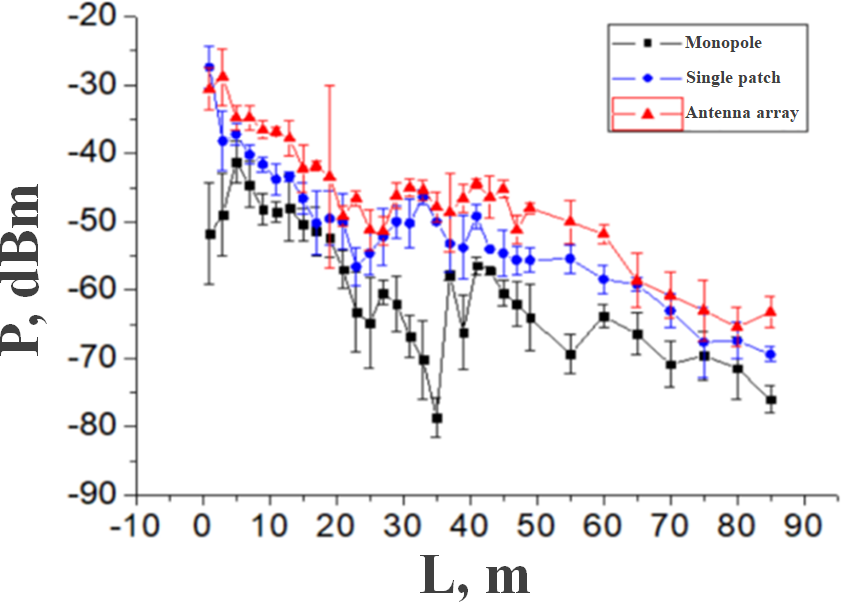
\includegraphics[width=\textwidth]{media/ict/image46}
   \end{subfigure}
   \caption*{Fig.6 - The dependence of received signal power on distance for three different antennas: monopole antenna, patch antenna, and antenna array, with the same transmission power level of 18 dBm at a frequency of 2.4 GHz}
\end{figure}

\begin{multicols}{2}
The radiation patterns of the antenna were plotted for three
frequencies: 2.2 GHz, 2.27 GHz, and 2.4 GHz. The maximum gain reaches 10
dBi, confirming the good directionality of the antenna. Moreover, the
radiation patterns exhibit notable similarity across the different
frequencies, indicating the stability of the antenna's directional
characteristics within the analyzed range.

The Figure 6 illustrates the variation in received signal strength
(RSSI) as a function of the distance between the transmitter and
receiver for three types of antennas: a monopole antenna (black line), a
single patch antenna (blue line), and a patch antenna array with four
elements (red line). The measurements were conducted with a consistent
transmission power level of 18 dBm at a frequency of 2.4 GHz. The
antenna array shows the best signal reception levels at all distances,
confirming its superiority over the other antenna types. It is also
observed that RSSI decreases with increasing distance for all antennas,
which aligns with the expected theoretical behavior.
\end{multicols}

\begin{figure}[H]
	\centering
	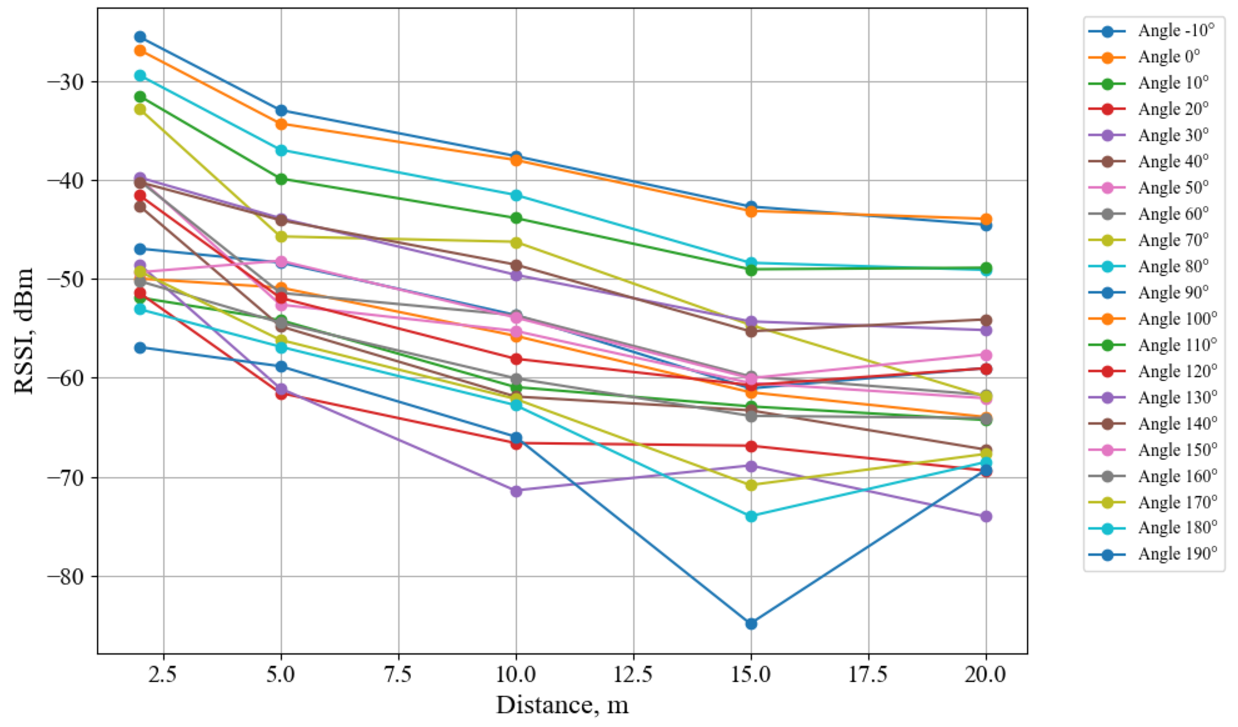
\includegraphics[width=0.7\textwidth]{media/ict/image47}
	\caption*{Fig.7 - RSSI dependence on distance for different measurement angles}
\end{figure}
\begin{figure}[H]
	\centering
	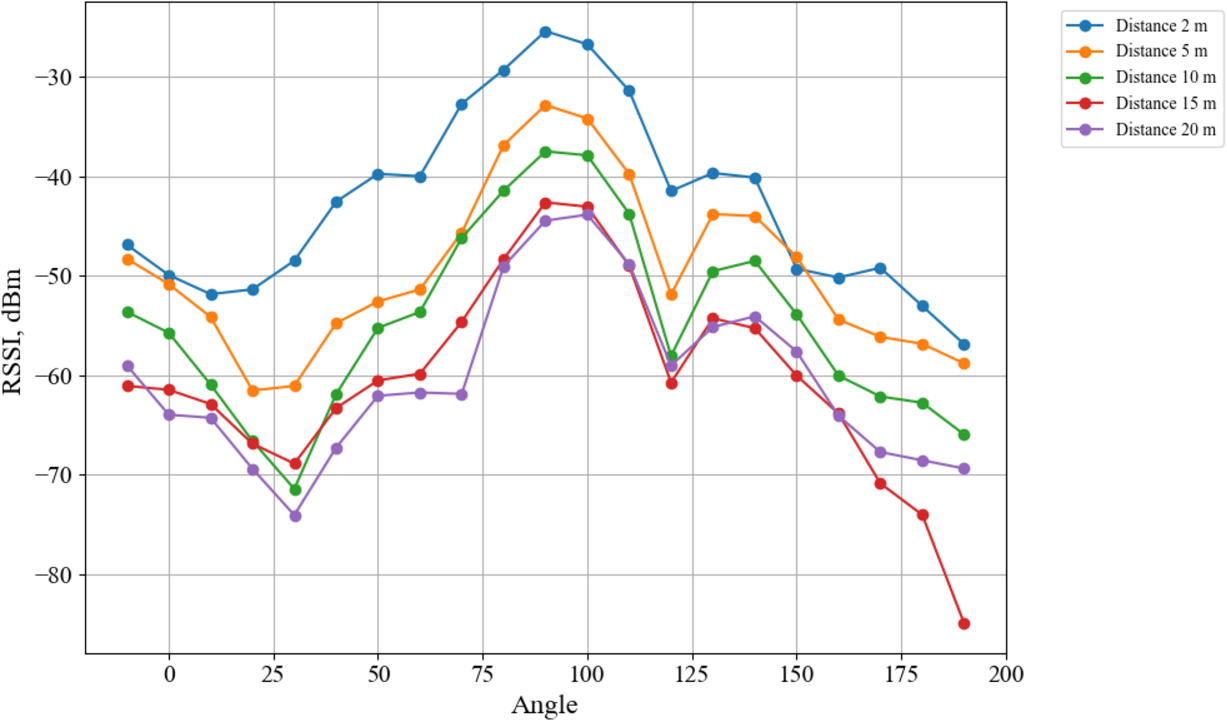
\includegraphics[width=0.7\textwidth]{media/ict/image48}
	\caption*{Fig.8 - RSSI dependence on the measurement angle for different distances}
\end{figure}

\begin{multicols}{2}
Figure 7 and 8 illustrates the variation in RSSI values as a function of
both distance and angular position. The graph provides a clear
visualization of how the RSSI by the antenna array changes under
different experimental conditions.

\emph{Distance Effect:} As the distance between the transmitter and the
antenna array increases, the RSSI value decreases consistently. This
behavior aligns with the fundamental principles of signal attenuation
over distance, where the signal strength weakens due to free-space path
loss.

\emph{Angle Effect:} The variation in RSSI across angular positions
reflects the directional sensitivity of the antenna array. Constructive
interference in the desired direction produces higher RSSI values, while
destructive interference in other directions reduces the signal
strength.

To enhance the understanding of how the Zigbee node' s
position can be accurately determined, machine learning techniques were
applied to process and analyze the collected RSSI and distance data.
During the experiments, data on RSSI values were collected at various
distances and angular positions relative to the antenna array.
Normalization of RSSI and distance values was performed to improve the
stability of model training and prevent bias due to features with large
scales. Then, a comparison of four machine learning
algorithms---XGBoost, Random Forest, Support Vector Machine, and
K-Nearest Neighbors - was conducted. The dataset was split into training
and testing sets. The models'{} performance was evaluated
using the following metrics: MAE, MSE, RMSE, and R² Score. The results
of model training and testing are presented in Tables 2 and 3,
respectively.
\end{multicols}

\tcap{Table 2 - Training results}
\begin{longtblr}[
  label = none,
  entry = none,
]{
  cells = {c},
  hlines,
  vlines,
}
\textbf{Machine			learning algorithms} & \textbf{MAE} & \textbf{MSE} & \textbf{RMSE} & \textbf{R²			Score}\\
XGBoost & 1,0778 & 2,8780 & 1,4091 & 0,9776\\
Random
			Forest & 1,4786 & 3,901165 & 1,9751 & 0,9656\\
Support
			Vector Machine & 7,2566 & 82,3409 & 9,0741 & 0,2748\\
K-Nearest
			Neighbors & 2,7802 & 15,3381 & 3,9163 & 0,8649
\end{longtblr}

\tcap{Table 3 - Testing results}
\begin{longtblr}[
  label = none,
  entry = none,
]{
  cells = {c},
  hlines,
  vlines,
}
\textbf{Machine			learning algorithms} & \textbf{MAE} & \textbf{MSE} & \textbf{RMSE} & \textbf{R²			Score}\\
XGBoost & 2,3568 & 3,9470 & 2,9994 & 0,9095\\
Random
			Forest & 3,1287 & 14,2804 & 3,7789 & 0,9002\\
Support
			Vector Machine & 9,0774 & 115,2343 & 10,734 & 0,2754\\
K-Nearest
			Neighbors & 3,2321 & 17,5434 & 4,1884 & 0,8896
\end{longtblr}

\begin{multicols}{2}
An analysis of the results showed that the XGBoost algorithm
demonstrated the best performance. It achieved the lowest error values
(MAE, MSE, RMSE) and the highest R² Score compared to the other models.
This indicates its strong generalization ability and high prediction
accuracy for this task. Other models, such as Random Forest, SVM, and
KNN, also showed competitive results, but their accuracy was lower,
especially SVM, which had the worst R² Score. Thus, XGBoost is the most
preferable choice for predicting RSSI values in this scenario.

The graphs in Figures 9 and 10 show a comparison of the actual and
predicted RSSI values \hspace{0pt}\hspace{0pt}for the training and test
datasets, confirming the high accuracy of the model in forecasting.

The decrease in RSSI values with increasing distance is a predictable
phenomenon, described by the free-space path loss model. However,
angular variation introduces additional complexity due to the
directional sensitivity of the antenna array, which creates nonlinear
dependencies.
\end{multicols}

\begin{figure}[H]
	\centering
	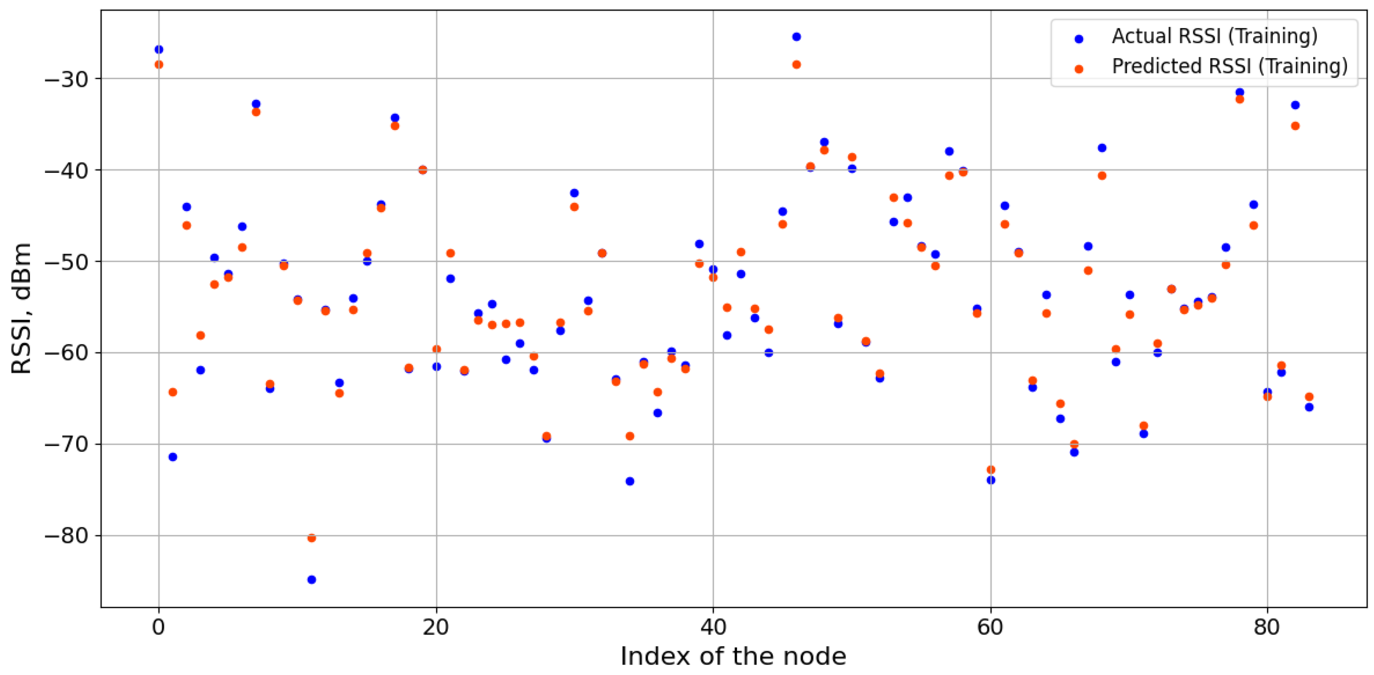
\includegraphics[width=0.8\textwidth]{media/ict/image49}
	\caption*{Fig.9 - Comparison of actual and predicted RSSI values on training data}
\end{figure}

\begin{figure}[H]
	\centering
	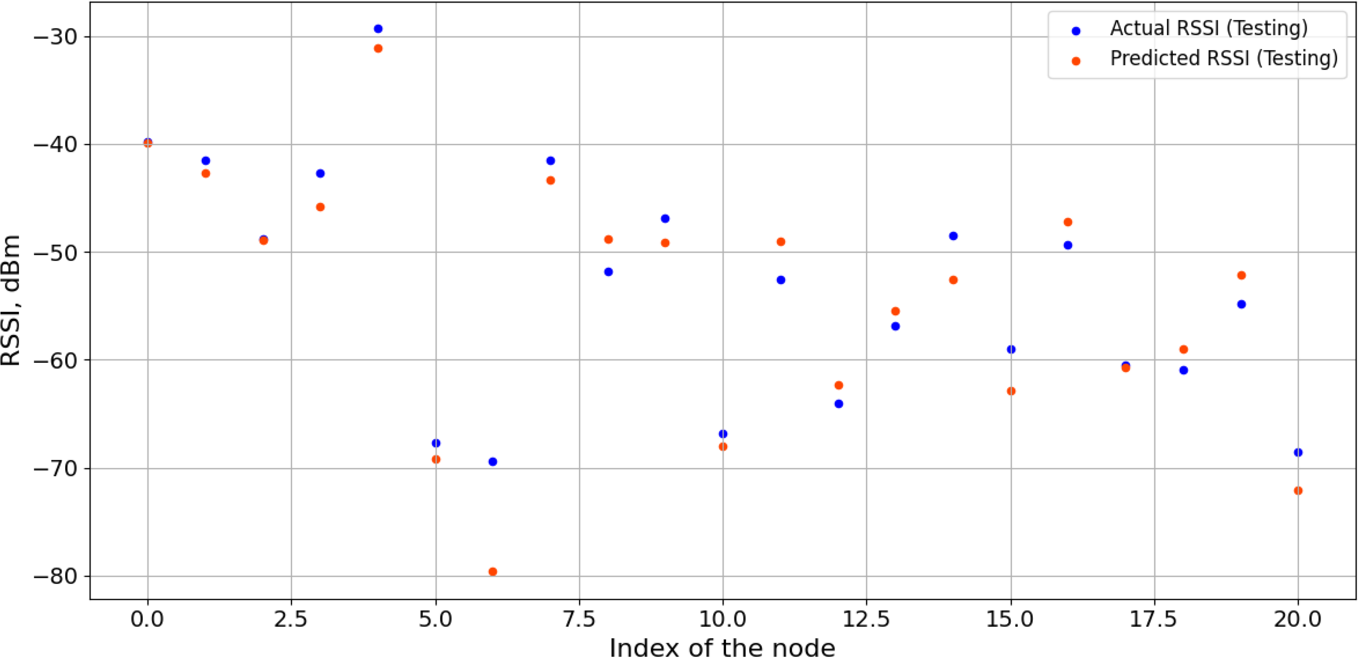
\includegraphics[width=0.8\textwidth]{media/ict/image50}
	\caption*{Fig.10- Comparison of actual and predicted RSSI values on testing data}
\end{figure}

\begin{multicols}{2}
{\bfseries Conclusion.} This article presents a single-anchor node
localization method that combines ZigBee technology, directional
antennas, and machine learning to provide a cost-effective, scalable,
and accurate solution for wireless sensor networks (WSNs). Experimental
results demonstrate that the use of a directional antenna array
significantly enhances signal reception, achieving a maximum gain of 10
dBi and reducing packet loss compared to monopole and single-band
antennas. The system effectively captures the relationship between RSSI,
distance, and angular positions, as evidenced by the consistent decrease
in RSSI values with increasing distance and their variation depending on
angular positions.

The XGBoost model trained on the experimental data outperformed other
machine learning algorithms, achieving a training R² of 97.76\% and a
testing R² of 90.95\%, with a training MSE of 2.878 and a testing MSE of
3.947. While the model performs well in controlled environments,
variability in testing highlights the need for further optimization. The
results demonstrate the potential of ZigBee-based single-anchor
localization systems as a viable alternative to traditional multi-anchor
setups, offering a reliable, energy-efficient, and cost-effective
solution for IoT and WSN applications requiring accurate and scalable
localization systems.

A single-anchor node localization system can be applied in industrial
facilities, smart buildings, medical institutions, and transportation
hubs to improve the accuracy of tracking objects and personnel.

In future research, we plan to conduct experiments in urban environments
and indoor spaces to study the impact of various interferences, such as
Wi-Fi and multipath signal propagation, on localization accuracy.

\emph{{\bfseries Financing.}} \emph{This research has been funded by the
Science Committee of the Ministry of Science and Higher Education of the
Republic of Kazakhstan (Grant AP19678552).}
\end{multicols}
\vspace{-1em}
\begin{center}
{\bfseries References}
\end{center}

\begin{references}
1. Osamy, W., Khedr, A. M., Salim, A., Al Ali, A. I., \& El-Sawy, A. A.
(2022). Coverage, deployment and localization challenges in wireless
sensor networks based on artificial intelligence techniques: a review.
IEEE Access.- 2022.-Vol.10.-P.30232-30257.
\href{https://doi.org/10.1109/ACCESS.2022.3156729}{DOI
10.1109/ACCESS.2022.3156729}

2. Xin, T. I. A. N., Guoliang, W. E. I., \& Gannan, W. A. N. G. (2022).
Review of wireless sensor network localization//Information and
Control.-2022.-Vol.51(1).-P.69-87.
DOI 10.13976/j.cnki.xk.2022.1177

3. Aly, H., Basalamah, A., \& Youssef, M. (2017). Accurate and
energy-efficient GPS-less outdoor \\localization// ACM Transactions on
Spatial Algorithms and Systems (TSAS).-2017.-Vol.3(2).-P.1-31.
\href{https://doi.org/10.1145/3085575}{DOI 10.1145/3085575}

4. Luo, J., Yin, Z., Gui, L., \& Yang, X. (2023, April). Accurate
localization for indoor and outdoor scenario by GPS and UWB
fusion. In 2023 9th International Conference on Control, Automation
and Robotics (ICCAR) (pp. 411-416). IEEE. DOI
10.1109/iccar57134.2023.10151723

5. Huang, Y. F., Chen, G. Y., \& Wu, H. C. (2024, July). An
Adaptive Three-Dimensional Indoor Positioning Using Multi-Anchor UWB
Wireless Communications. In 2024 International Conference on Consumer
Electronics-Taiwan (ICCE-Taiwan) (pp.521-522). IEEE.
DOI \\10.1109/ICCE-Taiwan62264.2024.10674260

7. Fu, Y. (2017). Single anchor node real-time positioning algorithm
based on the antenna array. \\International journal of distributed sensor
networks.-~2017-vol.13(5).-P.15501477177
DOI \\10.1177/1550147717709963

8. Wang, Ren, et al. Single-antenna super-resolution positioning with
nonseparable toroidal pulses.// \\Communications
Physicsю-2024.-Vol.7(1).-Num.356.
DOI \href{http://dx.doi.org/10.1038/s42005-024-01850-z}{10.1038/s42005-024-01850-z}

9. Groth, M., Nyka, K., \& Kulas, L. (2021). Calibration-free
single-anchor indoor localization using an ESPAR antenna// Sensors.-
2021. -Vol.21(10).- P.3431. \href{https://doi.org/10.3390/s21103431}{DOI
10.3390/s21103431}

10. Schmidt, S. O., Cimdins, M., John, F., \& Hellbrück, H. SALOS-A UWB
Single-Anchor Indoor \\Localization System Based on a Statistical
Multipath Propagation Model// Sensors.-2024.-Vol.24(8). -P.2428.
\href{https://doi.org/10.3390/s24082428}{DOI 10.3390/s24082428}

11.Wang, Z., Liu, M., \& Zhang, Y. (2019, October). Mobile localization
in complex indoor environment based on ZigBee wireless network//
Journal of Physics: Conference Series .-2019.-Vol. 1314(1):
012214). IOP Publishing. DOI 10.1088/1742-6596/1314/1/012214

12. Latina, M. A. E., Reyes, A., \& Rollon, E. M. (2022, February).
Optimization of RSSI-based Zigbee indoor localization system for
determining distances between unknown nodes. In 2022 First International
Conference on Electrical, Electronics, Information and Communication
Technologies (ICEEICT) (pp.1-6). IEEE. DOI
10.1109/ICEEICT53079.2022.9768601

13. Kimoto, R., Ishida, S., Yamamoto, T., Tagashira, S., \& Fukuda, A.
(2019). MuCHLoc: Indoor ZigBee localization system utilizing
inter-channel characteristics. Sensors, 19(7), 1645. DOI
10.3390/s19071645

14. Chen, T., \& Guestrin, C. (2016, August). Xgboost: A scalable tree
boosting system. In Proceedings of the 22nd acm sigkdd international
conference on knowledge discovery and data mining (pp.785-794). DOI
10.1145/2939672.2939785
\end{references}

\begin{authorinfo}
\hspace{1em}\emph{{\bfseries Information about the authors}}

Zholamanov B.N. - PhD student, Al-Farabi Kazakh National
University, Almaty, Kazakhstan, e-mail: \\zholamanov.batyrbek@kaznu.kz;

Nurgaliyev M.K. - PhD, Al-Farabi Kazakh National University, Almaty,
Kazakhstan, e-mail: \\madiyar.nurgaliyev@kaznu.edu.kz;

Bolatbek A.B. - PhD student, Al-Farabi Kazakh National University,
Almaty, Kazakhstan, e-mail: \\bolatbek.askhat@kaznu.kz;

Kopbay K.T. - PhD student, Al-Farabi Kazakh National University, Almaty,
Kazakhstan, e-mail: \\kopbay\_kymbat2@kaznu.edu.kz;

Kozhabek D.A. - master student, Al-Farabi Kazakh National University,
Almaty, Kazakhstan, e-mail: \\kozhabek\_dariga1@kaznu.edu.kz;

\hspace{1em}\emph{{\bfseries Авторлар туралы мәлімет}}

Жоламанов Б.Н. - PhD студент, әл-Фараби атындағы Қазақ Ұлттық
Университеті, Алматы, Қазақстан, e-mail: \\zholamanov.batyrbek@kaznu.kz;

Нұрғалиев M.K. - PhD, әл-Фараби атындағы Қазақ Ұлттық Университеті,
Алматы, Қазақстан, e-mail: \\madiyar.nurgaliyev@kaznu.edu.kz;

Болатбек А.Б. - PhD студент, әл-Фараби атындағы Қазақ Ұлттық
Университеті, Алматы, Қазақстан, e-mail: \\bolatbek.askhat@kaznu.kz;

Көпбай Қ.Т. - PhD студент, әл-Фараби атындағы Қазақ Ұлттық Университеті,
Алматы, Қазақстан, e-mail: \\kopbay\_kymbat2@kaznu.edu.kz;

Қожабек Д.А. - магистрант, әл-Фараби атындағы Қазақ Ұлттық Университеті,
Алматы, Қазақстан, e-mail: \\kozhabek\_dariga1@kaznu.edu.kz.
\end{authorinfo}
